\documentclass[12pt,a4paper]{article}
\usepackage[latin1]{inputenc}
\usepackage{fullpage}
\usepackage{color}
\usepackage{amsmath}
\usepackage{amsfonts}
\usepackage{amssymb}
\usepackage{hyperref}
\usepackage{graphicx}
\usepackage{url}

\title{BLAS to CUBLAS Transformation:\\
		Report for COMPOSE-HPC Project.}
\author{Ajay Panyala \\[1.8ex]
Louisiana State University\\[1.8ex]
ajay@csc.lsu.edu}
\date{Oct 12, 2011}

\begin{document}
\maketitle
\section{Introduction}
Many compute intensive scientific applications make heavy use of tuned numerical 
libraries such as BLAS \cite{BLAS}. Equivalent libraries such as CUBLAS \cite{CUBLAS} provide means to harness the computational resources of GPUs thereby achieving significant performance improvements.  Replacing the original library calls in existing applications with the GPU version is tedious and needs more thought due to the additional complication of adding memory management and other supporting code to make the GPU library calls work as expected and thereby reap the performance benefits.

This document describes an annotation guided transformation that transforms C/ C++ 
source code that use BLAS calls into CUDA code containing CUBLAS calls along
with the appropriate memory management and support code. The transformation
is built using the ROSE compiler framework \cite{ROSE} and Coccinelle \cite{Coccinelle},
a term rewriting system.

\section{Overview}
An overview of the steps involved in the transformation is shown
in Figure~\ref{fig:overview}. A simple translator built using the
ROSE compiler is run on the input source code provided and produces
a new source code wherein some terms are rewritten such that 
the overall behaviour of the original input source does not change. 
The new source code is then passed to the automated annotation stage
where all the BLAS calls in the code are annotated if the user desires to 
transform all the BLAS calls in his code to CUBLAS calls. If the user desires
to transform only a few BLAS calls, the automated annotation stage is skipped and 
the user is expected to manually annotate the BLAS calls he desires to transform. 
The annotated input source is then passed to the transformation stage 
where the actual transformation takes place and the appropriate CUDA 
code is generated.


\begin{figure}
{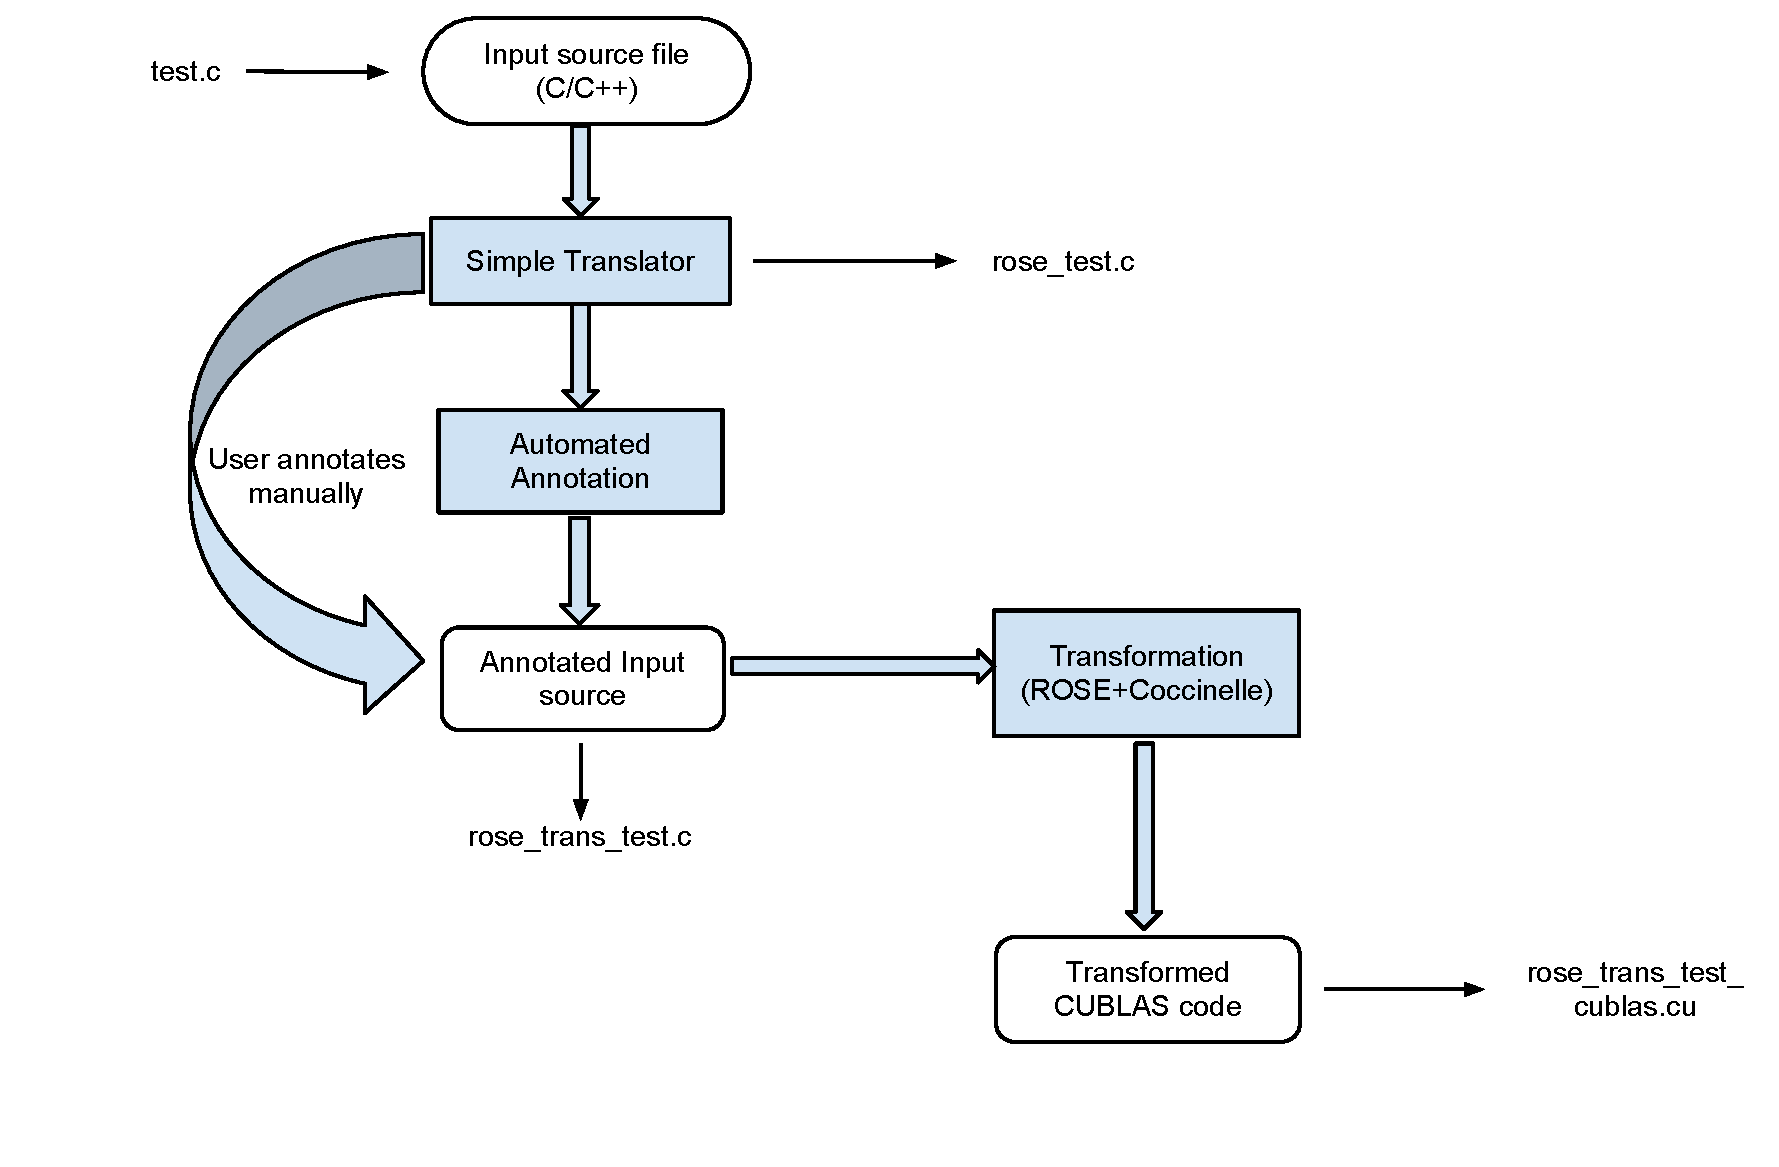
\includegraphics[width=15cm]{transOverview.pdf}} 
\caption{\label{fig:overview}%
Overview of the Transformation.}
\end{figure}

\section{Transformation Details}
This section explains each stage of the transformation in more detail.

\subsection{Input source code}
\label{blascall}

The annotation associated with a BLAS call
must be placed in juxtaposition with the BLAS
calls to which they are intended to apply. An example follows
(annotation shown within comments):\vspace{2ex} 
\newline {\color{red}$/*$\% BLAS\_TO\_CUBLAS prefix = device1 $*/$} 
\newline $cblas\_sgemm(CblasRowMajor, CblasNoTrans, CblasNoTrans,$ 
\newline \hspace*{21mm} $ n, n, n, 1.0,\&a[0],n, \&b[bi+ci],n, 1.0, c,n);$

The value of \textit{prefix} could be any valid identifier names.
New variables are introduced into the transformed code and 
the names of these variables are prefixed by this user provided 
identifier names to avoid name clashes with existing variables 
in the original code.

\subsection{Simple Translator}
The simple translator is built using ROSE. It contains a call to the ROSE frontend which generates the abstract syntax tree (AST) ROSE uses for the input source provided, and a call to backend unparses the AST to generate the same source code with some terms rewritten in
such a way that the overall behaviour of the input source code provided does not change.

The need for the Simple Translator arises because the transformation tries to extract information (such as array references) from the annotated BLAS call for the sake of generating a Coccinelle patch later to transform the given input source. The patch contains the rewritten terms, which would not match with the terms in the original input source and the transformation would not be applied because Coccinelle would not find the BLAS call to be matched (since it is looking for the rewritten BLAS call). For example
consider the BLAS call in \ref{blascall}. When ROSE parses this code and builds the AST and
we try to extract the array names so that we can write a patch using Coccinelle to match
the BLAS call and replace it with the appropriate CUDA code. The rewritten BLAS call looks like \vspace{2ex} 
%\newline {\color{red}$/*$\% BLAS\_TO\_CUBLAS prefix = device1 $*/$} 
\newline $cblas\_sgemm(CblasRowMajor, CblasNoTrans, CblasNoTrans,$ 
\newline \hspace*{21mm} $ n, n, n, 1.0,{\color{red} (a + 0)},n,{\color{red} (b + (bi + ci))}, n,1.0,c,n);$ \vspace{2ex} 
\newline The array reference {\color{red} \&a[0]} in the BLAS call in \ref{blascall} and {\color{red} (a + 0)} here mean the same thing. When ROSE builds the AST and
the transformation tries to unparse it in order to determine the array references, the array references are rewritten without affecting the behaviour of the input source code provided. If the Simple Translator is not used to generate this code first, the Coccinelle patch generated would try to match the rewritten BLAS call (for replacing it with CUDA code) with the one in \ref{blascall} and would fail in doing so because the code pattern is different.

\subsection{Automated Annotation}

The source code from simple translator is fed to the automate annotation stage.
If the user desires to annotate all the BLAS calls he can leave it upto the transformation to 
do this. A Coccinelle patch takes care of this. It annotates all BLAS calls present in the input source and with each annotation a unique prefix is generated. This prefix cannot be specified by user as of now, but support for specifying the prefix will be added soon.
Annotations can be added manually by the user only to those BLAS calls that the user
desires to transform. In this case the automated annotation stage is skipped.

\subsection{Transformation}
The annotated source is passed on to the actual transformation phase.
A new header (\textit{cublas.h}) needs to be inserted into the transformed code
because the transformed code would be using the CUBLAS API. It is inserted before
the first header include found in the input source provided.

To understand the details of the actual transformation consider again the \textit{sgemm} BLAS call:\vspace{2ex} 
%\newline {\color{red}$/*$\% BLAS\_TO\_CUBLAS prefix = device1 $*/$} 
\newline $cblas\_sgemm(CblasRowMajor, CblasNoTrans, CblasNoTrans,$ 
\newline \hspace*{24mm} $ n, n, n, 1.0,{\color{red} (a + 0)},n,{\color{red} (b + (bi + ci))}, n,1.0,c,n);$ \vspace*{2ex}
\newline The array references are matched explicitly to avoid ambiguity among the different
\textit{sgemm} calls in the input source. If we do not explicitly match the array references and rather match whatever is there, all the \textit{sgemm} calls in the input source get transformed even if they are not annotated. As for the rest of the arguments they are matched with whatever is there, except that for those cases where calls use the CBLAS API, there is some more work involved which is explained in the following text. If we have two \textit{sgemm} calls that are exactly the same (have the exact same arguments) both are transformed even if only one of them is annotated. 

The steps in the transformation stage could be summarized as follows. The array references are extracted from the above sgemm call using ROSE API. The storage order and transpose options are also determined because this call uses the CBLAS API which allows specifying row-major storage for arrays and CUBLAS assumes only column-major storage for arrays. These options are defined as enumerated types in the CBLAS API. CUBLAS routines accept character constants for transpose options. Hence the transformation cannot simply use the transpose options that are present in the regular BLAS calls using the CBLAS API with CUBLAS calls. The transformation would need to determine what the transpose options are so that it could pass the equivalent options that conform with the CUBLAS API. It may not be possible  to determine them always since variables containing the transpose and storage-order options might be passed as arguments. In such cases the logic for determining and passing the equivalent options to the CUBLAS call is generated as part of transformed code. If the input source uses FORTRAN BLAS API (which assumes column-major storage for arrays), then the options from the BLAS call could be passed as is to the CUBLAS call that is going to be generated. A Coccinelle patch is generated for each annotated BLAS call. A single patch file per input source file containing patches for all the annotated BLAS calls is generated. These patches specify a code pattern to be matched and a replacement pattern to be substituted which are processed by Coccinelle. The Cocinelle patch (complete patch not shown) for the BLAS call being discussed is as follows: 
\begin{verbatim}
@disable paren@ 
expression order,transA,transB;  
expression m,n,k,alpha,lda,ldb,beta,ldc; 
@@ 
- cblas_sgemm(order,transA,transB,m,n,k,alpha,
(a + 0), lda, (b + (bi + ci)),ldb,beta,c,ldc); 

+ /* Allocate device memory */ 
+ /* Copy matrices to device */ 
+ /* Storage Order Warning */ 

+ /* CUBLAS call */ 
+ cublasSgemm('N','N',m,n,k,alpha,device1_A,lda,
              device1_B,ldb,beta,device1_C,ldc); 
              
+ /* Copy result array back to host */ 
+ /* Free device memory */ 
\end{verbatim}

\section{Transformed Code}
\begin{itemize}
  \item Depending on the type of BLAS library being used, the non-standard headers and
external function calls in the input source (C sources only) need to be enclosed within
\textit{extern $``$C $"$} and this needs to be done by the user. The reason is the transformed
cuda code when compiled with the nVidia C compiler (nvcc), the external libraries are
linked using g++.

\item If the original input source uses the CBLAS API and row-major storage
for arrays is specified the transformed code would have a warning nested in a comment above the
CUBLAS call saying the original BLAS call assumed row-major storage for the arrays.

  \item Certain BLAS routines listed below are not handled by the transformation since CUBLAS
does not provide them. They are listed as follows:
  \begin{itemize}
  \item BLAS 3 -$>$ \{c,z\}gemm3m, \{sc,dz\}gemm, \{sc,dz\}gemv (Intel MKL only)
  \item BLAS 2 -$>$ \{s,d\}gem2vu, \{c,z\}gem2vc (Intel MKL only)
  \item BLAS 1 -$>$ \{ds,sds\}dot, \{d,s\}cabs1 
  \item CUDA BLAS library provides routines for {rotg, rotmg}
 \newline for completeness sake and are run on the CPU.
  \end{itemize}

\end{itemize}

\section{Future Work}
  \begin{itemize}
 \item The transformation currently works under an unrealistic assumption that
the memory available on the GPU is atleast equal that of the CPU memory, which
is not always true in practice. Another way to look at this is the transformation 
assumes that the computation fits within GPU memory. This assumption would
be removed in later iterations of the transformation by generating code for moving data between CPU 
and GPU memory if the entire computation would not fit in GPU memory.
 \item The transformation also does not take advantage of multiple GPUs (when
available) in a system since the CUBLAS library does not auto-parallelize
across multiple GPUs.
 \item Currently the transformation does not provide support for task parallelism.
Task parallelism involves performing two or more completely different tasks 
in parallel. This approach is especially useful when the computation performed 
by a single task is relatively small and is not enough to fill the GPU with work.
Such tasks could be identified by the user and could be made explicit through
an annotation so that the transformation knows which tasks could be executed 
in parallel to efficiently utilize the GPU resources.
\item Use name mangling provided by ROSE to avoid name clashes instead of
the user having to specify a prefix for new variables in transformed code.
\item The transformation currently follows the CUBLAS library version 3.2 and
hence lacks the new features provided by version 4.0. Later iterations of the transformation would include those new features for generating more efficient
CUDA code.

\end{itemize}
  
\section{Code Availability}
The sources for the transformation are available at \url{http://sourceforge.net/projects/compose-hpc}. 
The sub-direcotry paul/demo/blas2cublas contains the source code and testcases
along with a README file with instructions for getting the transformation working
on your machine.


\bibliographystyle{IEEE}
\bibliography{references}

\end{document}
